\documentclass{article}

\usepackage[margin=1in]{geometry}
\usepackage[utf8]{inputenc}
\usepackage[parfill]{parskip}
\usepackage{amsmath}
\usepackage{amsfonts}
\usepackage{caption}
\usepackage{graphicx}
\usepackage{subcaption}
%\usepackage{subfigure}

\title{Learning from (multiple) demonstrations through robust trajectory transfer}
\author{Alex Lee, Dylan Hadfield-Menell, Eric Tzeng, Sandy Huang}
\date{}

\renewcommand{\thesection}{\Roman{section}}
\renewcommand\thesubsection{\Alph{subsection}}
%\renewcommand{\thesubsection}{\thesection.\Roman{subsection}}

\begin{document}

\maketitle

\begin{abstract}
We investigate extensions to a previously presented method of learning from demonstrations via trajectory transfer. We present a variety of techniques such as unified optimization of non-rigid registration and trajectory feasibility, as well as the incorporation of surface normals, and show that such techniques definitively improve the robustness of the final trajectory found. We also propose an improved method for selecting trajectories from a bank of demonstrations which uses the structure of the provided demonstrations to avoid unexplored areas of the state space. We demonstrate that our selection strategy improves the success rate in an autonomous knot-tying scenario, enabling a robot to succeed in configurations where simple nearest-neighbor demonstration selection fails.
\end{abstract}

\section{Introduction}

Robots often have to perform a given task in a variety of scenarios, making it impractical or even impossible to individually specify trajectories for all possible scenarios. \emph{Learning from demonstrations} is an approach that enables robots to generalize from demonstrations of manipulation tasks in order to perform them in new scenarios. We explore approaches that make this generalization via trajectory transfer more robust and improve its application to multiple demonstrations.

To improve the robustness of trajectory transfer, we use a unified optimization to determine a feasible trajectory in the new scenario. Instead of Schulman et al.'s state-of-the-art two-step approach~\cite{Schulmanetal_ISRR2013}, which first finds the optimal smooth low-cost registration between the scenes and then a feasible trajectory, we propose optimizing for both at once. We show this unified approach generalizes demonstrations better by satisfying the ultimate goal -- finding a feasible trajectory in the new scene that has a low-cost registration to the demonstration scene and trajectory.

We also incorporate surface normals into the optimization in order to improve robustness. Without explicitly specifying surface normal correspondences, in order to preserve smoothness the optimal warping function often does not match normals. However, this is undesirable in situations such as suturing, where the robot's angle of approach to the surface is crucial to its performance of the task.

When there are multiple demonstrations of a task, we improve demonstration selection through simulation and forward search. We simulate potential new trajectories in order to avoid selecting demonstrations that drive us into unrecoverable configurations. We identify unrecoverable states by clustering demonstrations with kernelized $k$-means and using cluster consensus among the $k$-nearest neighbors according to registration cost.

\section{Background}

\subsection{Trajectory Optimization with Sequential Convex Programming}

\subsection{TPS-RPM}

Schulman et al.'s state-of-the-art approach to learning from demonstrations~\cite{Schulmanetal_ISRR2013} calculates the new trajectory by first using a modified thin plate spline robust point matching (TPS-RPM) algorithm~\cite{ChuiR00} to calculate a non-rigid scene registration that maps points from the demonstration scenario to the new scenario. TPS-RPM alternates between (1) estimating correspondences between the two scenes' point clouds and (2) fitting the optimal thin plate spline transformation based on these estimated correspondences. Then, the mapping function is applied to the demonstration trajectory in order to obtain a potential trajectory for the new scenario. This potential trajectory does not incorporate collision avoidance and joint limits, so trajectory optimization is then used to incorporate these constraints. The hope is that the resulting trajectory will incorporate variations in the environment and thus succeed in performing the desired manipulation.

This method is effective at generalizing expert demonstrations to new, unseen scene configurations. However, because the warp function discovery and trajectory optimization are performed in two separate steps, in some cases the final feasible trajectory can ``contradict'' the discovered warp, for instance by bending a trajectory in the opposite direction of the warp. Our method of jointly optimizing the warp and the trajectory avoids these contradictions and results in trajectories that are better conditioned for success.

% TODO: edit this paragraph pls
This method of learning from demonstrations has also been applied to the task of suturing \cite{Schulmanetal_IROS2013}. Schulman et al.'s two-step approach often finds warps that fail to preserve surface normals. This does not preserve much of the geometric structure of the original scene and frequently leads to execution failures. To address this, we investigate the problem of incorporating correspondences on surface normals in this framework. We present preliminary results that show promise in this approach.

%% John's TPS-TrajOpt
%% - \cite{Schulmanetal_ISRR2013} lfd paper
%% - \cite{Schulmanetal_IROS2013} suturing paper <== we're not citing this one yet and I think we should
%% - \cite{ChuiR00} TPS-RPM paper
%% Normals
%% - \cite{BooksteinGreen} normals I think <==== this one probably needs to go in future work
%% Prior work on clustering/lookahead
%% - \cite{Dhillon2004} kernelized k-means, although does this really go here?!

\section{Unified Optimization}

We propose an optimization problem which seeks to jointly optimize for both a smooth warping function (based on TPS) and a feasible trajectory. The problem we solve is

\begin{equation}
\begin{aligned}
  & \min_{f,\Theta,\Phi}
  & & \sum_{i=1}^m ||\mathbf{x}_t^{\emph{(i)}} - f(\mathbf{x}_s^{\emph{(i)}})||_2^2 + \sum_{j=1}^n ||\mathbf{\phi}_t^{\emph{(j)}} - f(\mathbf{\phi}_s^{\emph{(j)}})||_2^2 + \lambda ||f||_{tps}^2 \\
  & \text{ s.t.}
  & & \mathbf{\phi}_t^{\emph{(j)}} = \text{ForwardKinematics}(\mathbf{\theta}^{\emph{(j)}}), \; j = 1, \ldots, n \\
  &
  & & \mathbf{\theta}^{\emph(j)} \text{ is feasible}, \; j = 1, \ldots, n
\end{aligned}
\end{equation}

$f$ is the TPS function that warps points from the source scene to the target scene, and $\Theta$ is composed of the robot's joint angles $\theta^{(j)}$ at each time step $j$ for a feasible trajectory in the target scene. Applying forward kinematics to each $\mathbf{\theta}^{\emph(j)}$ gives the gripper pose $\mathbf{\phi}_t^{\emph{(j)}}$ at time step $j$. The first summation is over the \emph{m} pairs of scene correspondences, and the second summation is over the \emph{n} time steps of the trajectory. $\forall i$, $\mathbf{x}_s^{\emph{(i)}}$ and $\mathbf{x}_t^{\emph(i)}$ each refer to a correspondence point in the source and target scene, respectively. $\forall j$, $\mathbf{\phi}_s^{\emph{(j)}}$ is the gripper pose at time step $j$ of the trajectory in the demonstration. $\lambda ||f||_{tps}^2$ is a regularization term that encourages the warping function $f$ to be smooth. This formulation is similar to the previous formulation in \cite{Schulmanetal_ISRR2013}, but it includes an extra trajectory-related term and trajectory feasibility constraints.

\subsection*{Experimental Results}

\begin{figure}[h!]
\centering
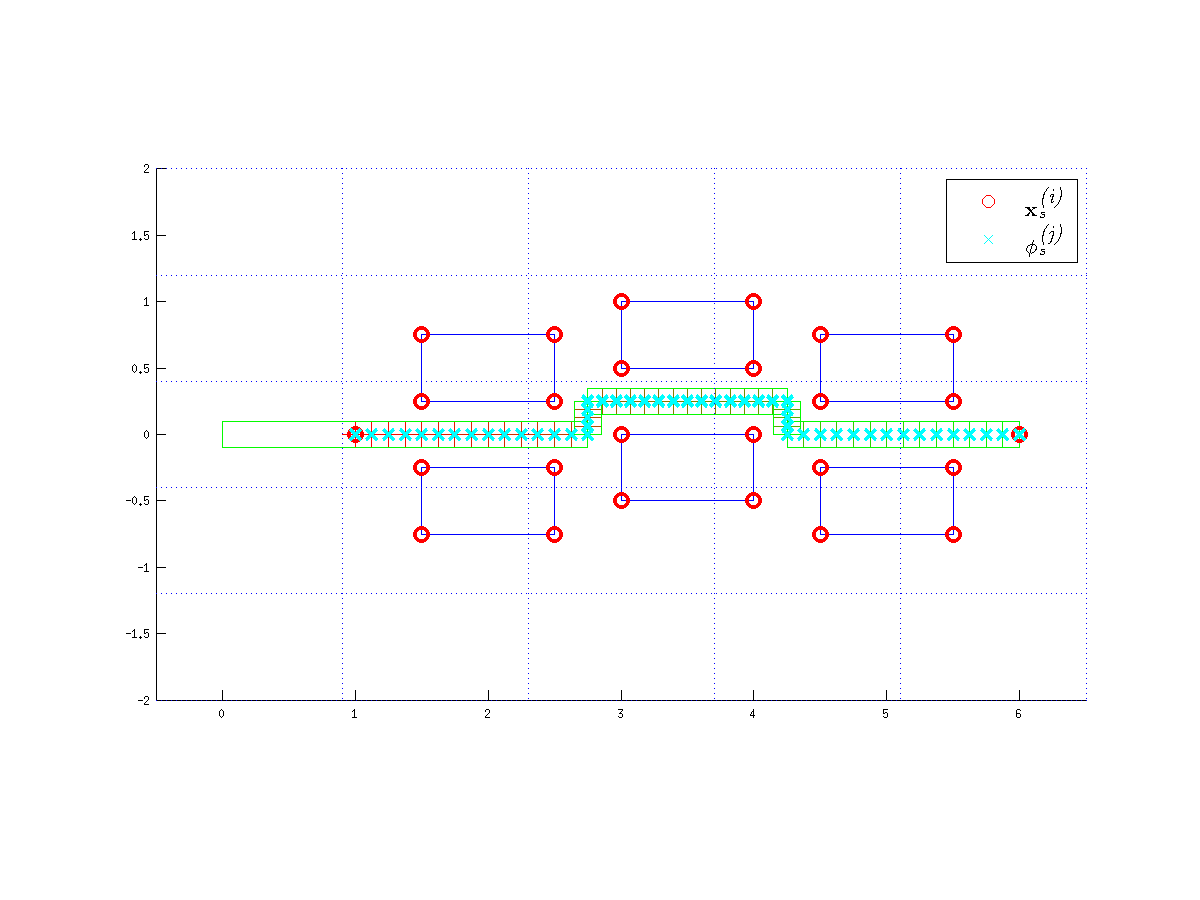
\includegraphics[width=0.5\textwidth]{scopey_demo}
\vspace{-1cm}
\caption{Demonstration trajectory for robot with telescoping links. The blue rectangles are the obstacles, the red points indicate the scene correspondence points, and the green outline and red line trace the trajectory of the robot.}
\label{fig:scopey_demo}
\end{figure}

\begin{figure}[h!]
\begin{subfigure}[b]{0.5\textwidth}
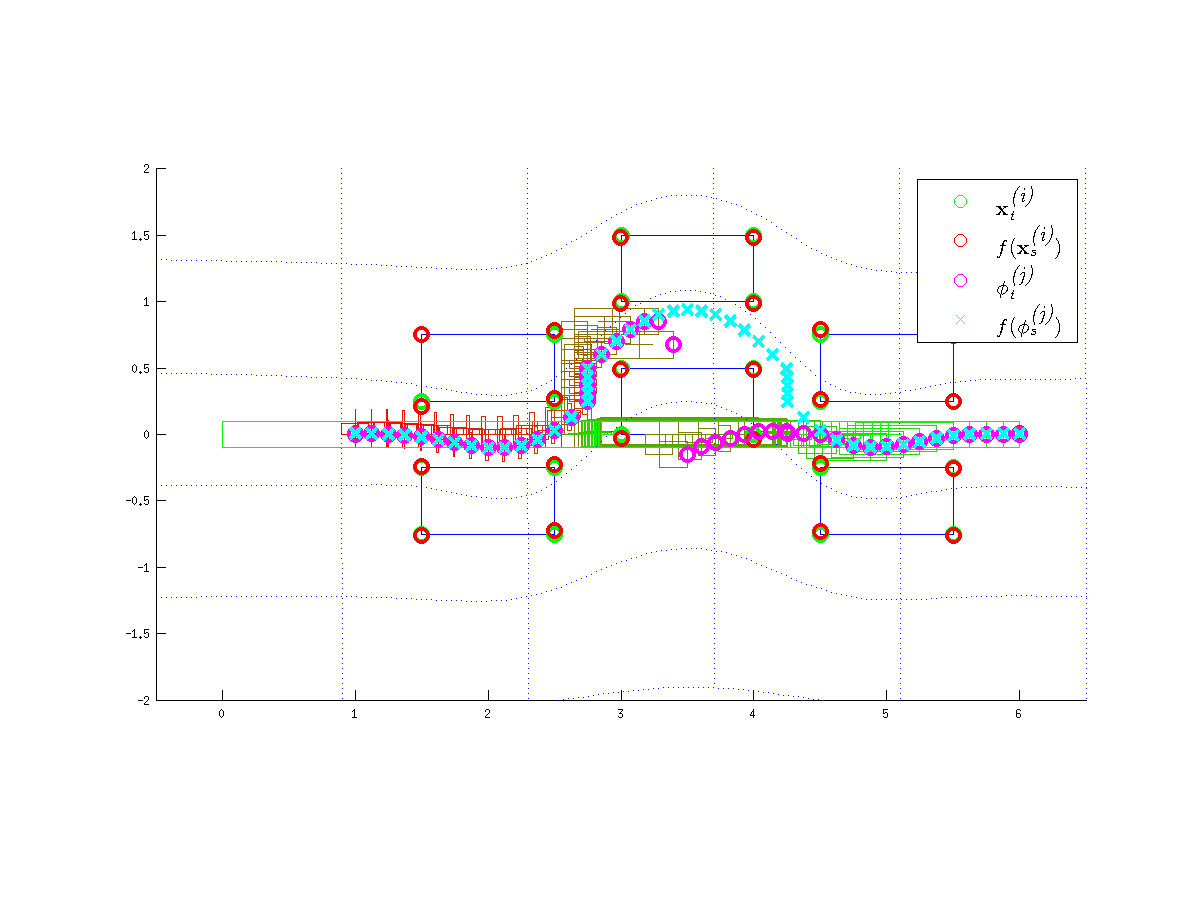
\includegraphics[width=\textwidth]{scopey_2step}
\vspace{-1.5cm}
\caption{}
\end{subfigure}
%\hspace{0.02\textwidth}
\begin{subfigure}[b]{0.5\textwidth}
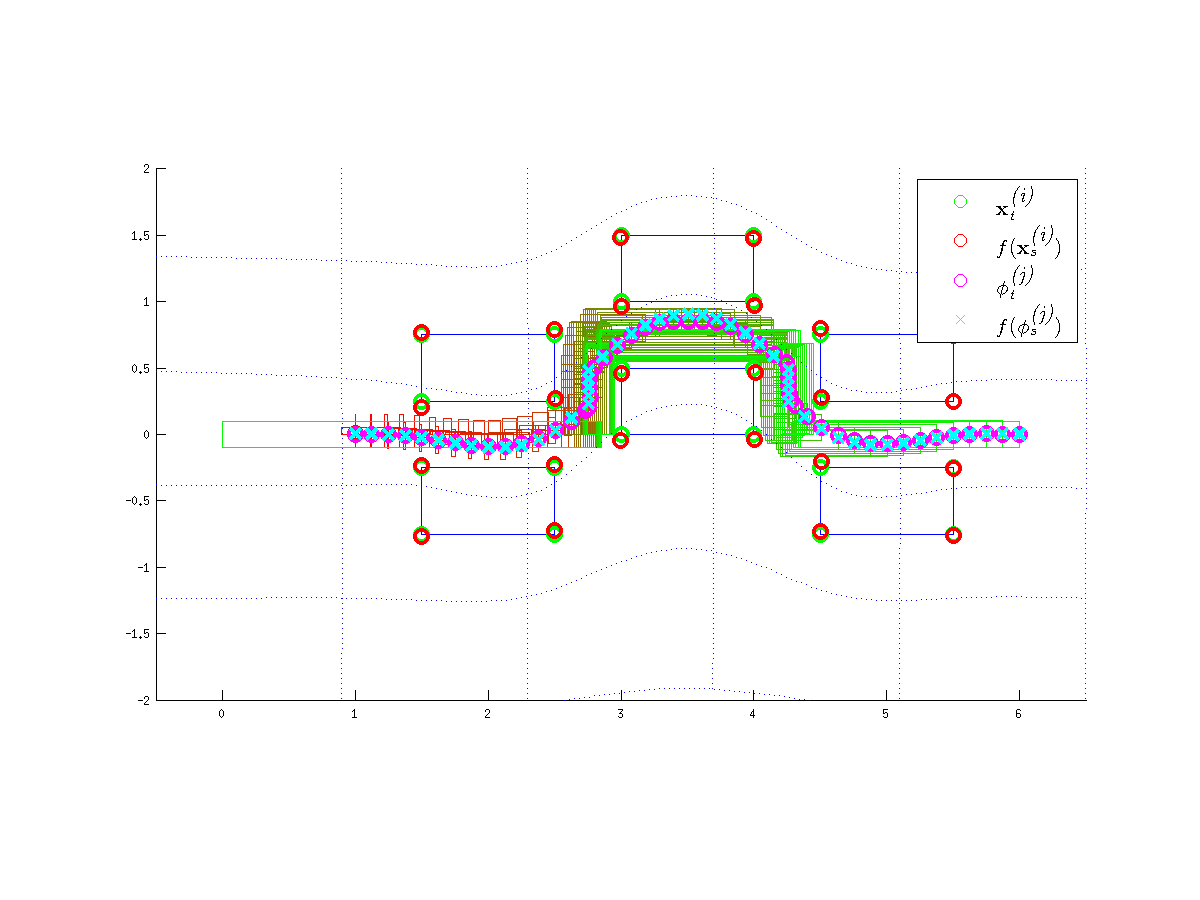
\includegraphics[width=\textwidth]{scopey_unified}
\vspace{-1.5cm}
\caption{}
\end{subfigure}
\caption{The warped blue grid shows the registration from the demonstration scene to the new scene, in which the two middle obstacles are shifted slightly upwards. (a) Two-step optimization does not find a feasible trajectory. (b) Unified optimization is able to find a feasible trajectory.}
\label{fig:scopey_results}
\end{figure}

Our unified optimization leads to improved performance over the two-step appraoch on two-dimensional tasks with pre-defined scene correspondences. For a 2D holonomic car, unified optimization results in trajectories that more smoothly navigate around obstacles. We also applied our formulation to a robot with five telescoping links (three horizontal links interconnected by two vertical links). In the demonstration (Figure~\ref{fig:scopey_demo}), we specify a trajectory for the robot to navigate through a tunnel formed by three pairs of rectangular obstacles. In the new scene, the middle pair of obstacles is shifted upwards. The two-step optimization is unable to find a feasible trajectory, whereas our unified optimization approach finds a feasible trajectory by finding a warping function that warps the scene more upwards around the middle pair of obstacles (Figure~\ref{fig:scopey_results}).

\section{Matching Surface Normals}

\begin{figure}[h!]
\centering
\begin{subfigure}[b]{0.9\textwidth}
\centering
\hspace{-0.7cm}
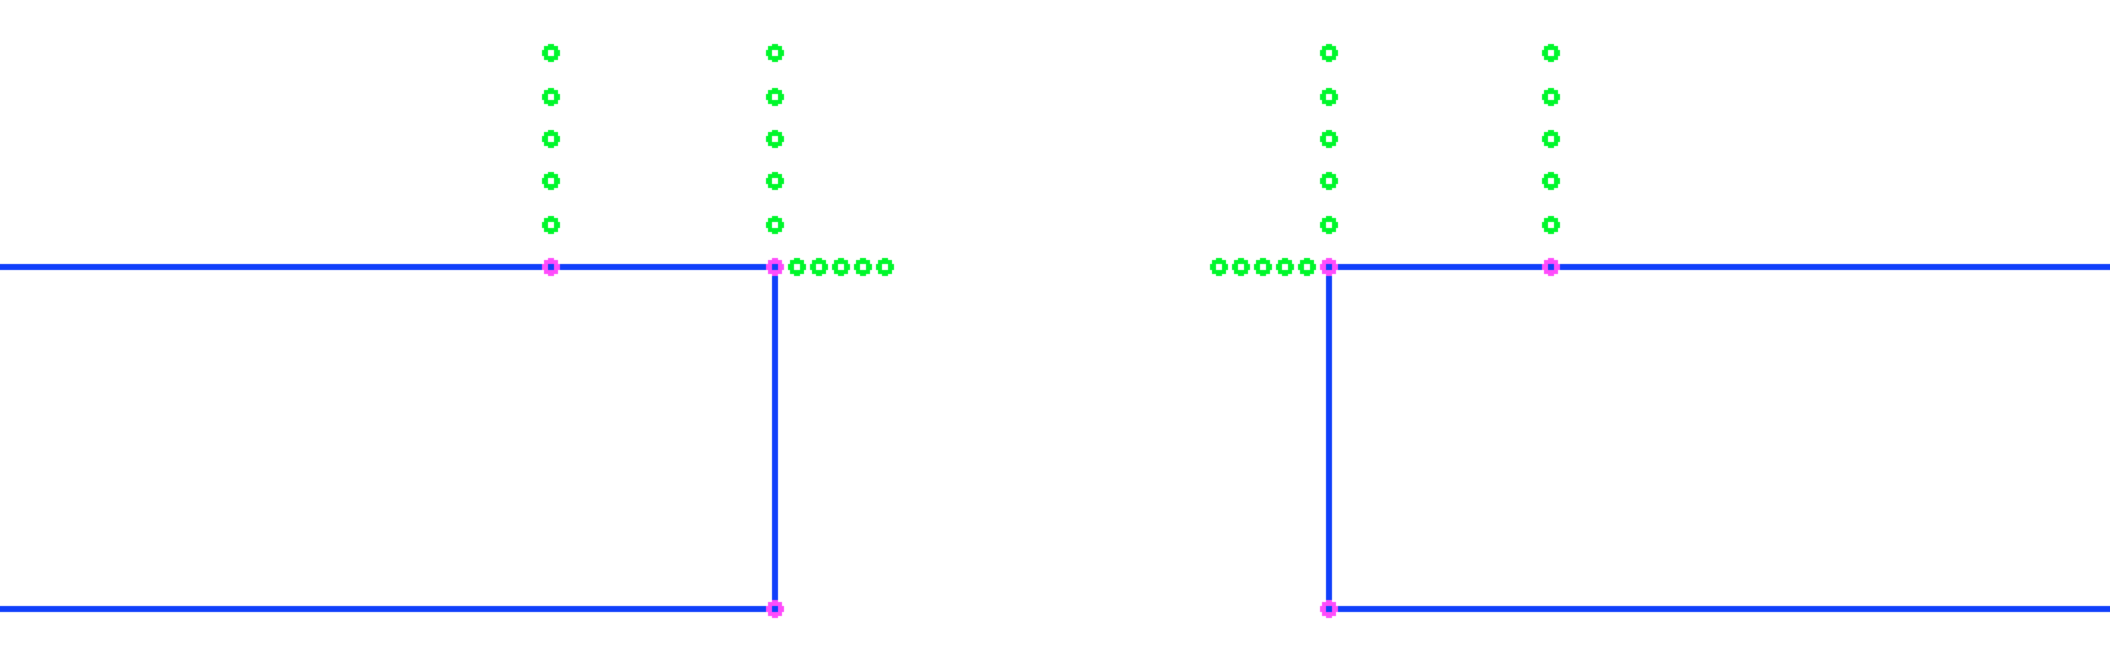
\includegraphics[width=8cm, height=3cm]{normals_points}
\end{subfigure}
\begin{subfigure}[b]{0.4\textwidth}
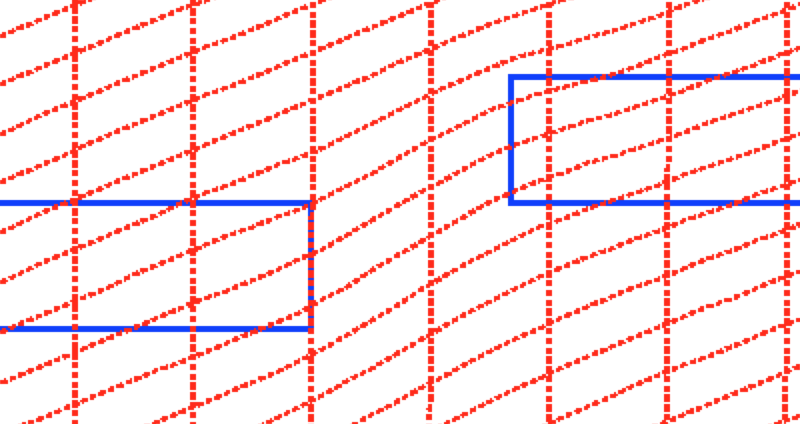
\includegraphics[width=6cm, height=3cm]{TPS_withoutnormals}
\caption{}
\end{subfigure}
\hspace{0.02\textwidth}
\begin{subfigure}[b]{0.4\textwidth}
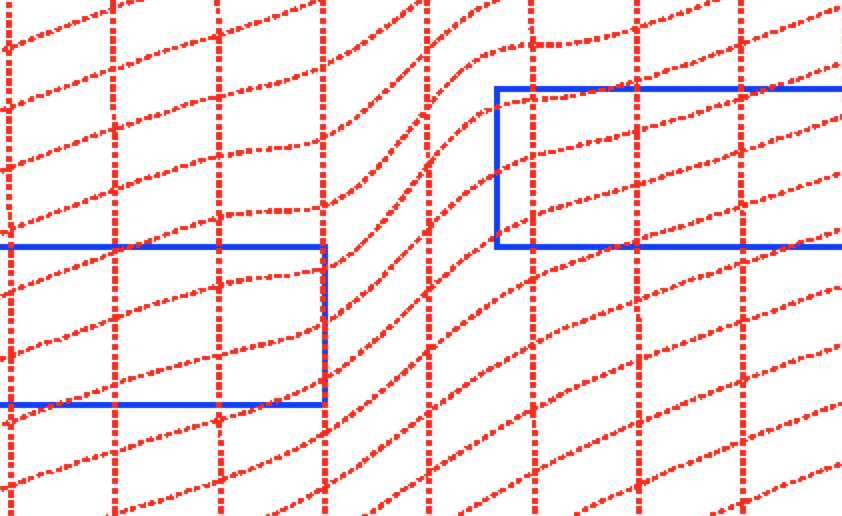
\includegraphics[width=6cm, height=3cm]{TPS_withnormals}
\caption{}
\end{subfigure}
\caption{The demonstration scene (top image) has two suturing pads aligned in the same horizontal plane. In the test scene (bottom two images) the right pad is shifted upwards. (a) Warp found by TPS using six pairs of correspondence points between the scenes, indicatd by the magenta points. (b) Warp found by TPS after adding in correspondence points along the relevant normals, indicated by the green points. The second warp is more likely to effectively generalize trajectories as it better captures the structure of scene.}
\label{fig:normals}
\end{figure}


\begin{figure}[h!]
\centering
\begin{subfigure}[b]{0.9\textwidth}
\centering
\hspace{-0.7cm}
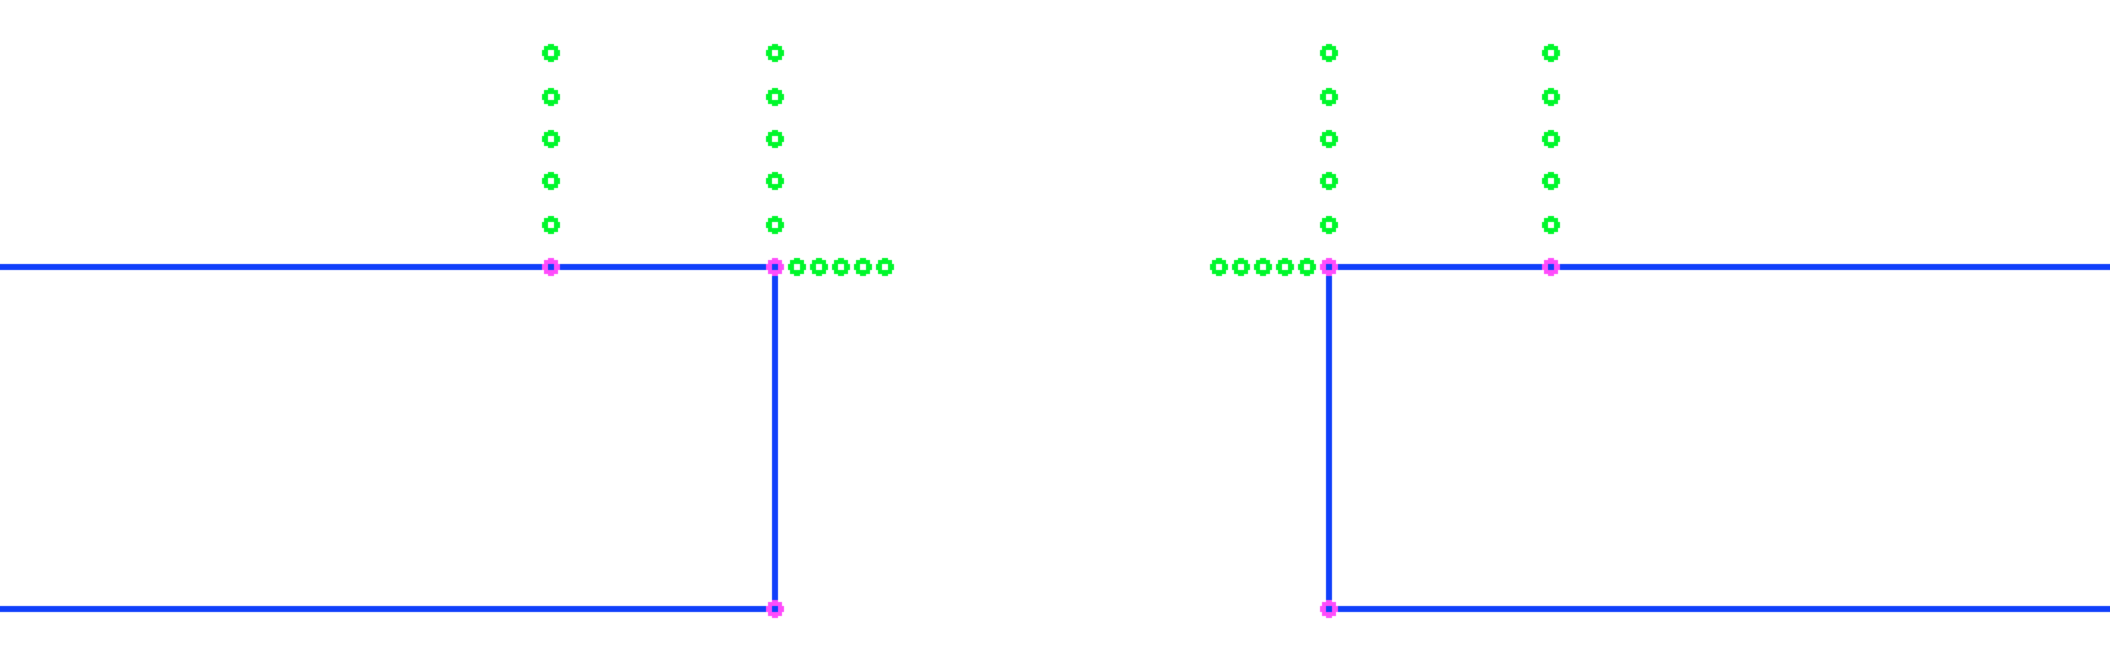
\includegraphics[width=8cm, height=3cm]{normals_points}
\end{subfigure}
\begin{subfigure}[b]{0.4\textwidth}
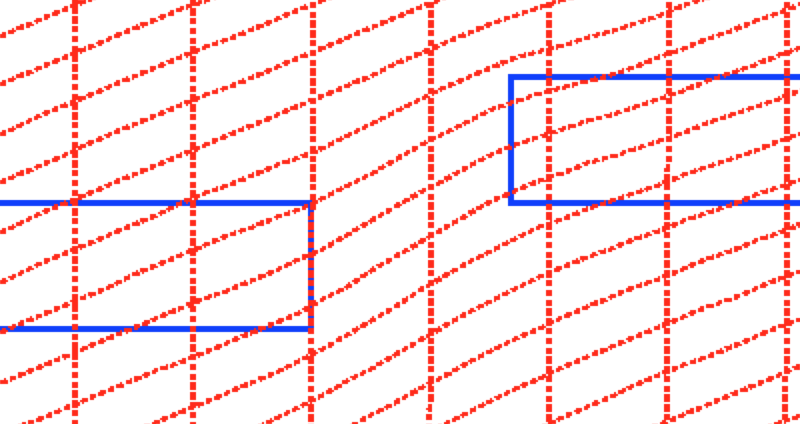
\includegraphics[width=6cm, height=3cm]{TPS_withoutnormals}
\caption{}
\end{subfigure}
\hspace{0.02\textwidth}
\begin{subfigure}[b]{0.4\textwidth}
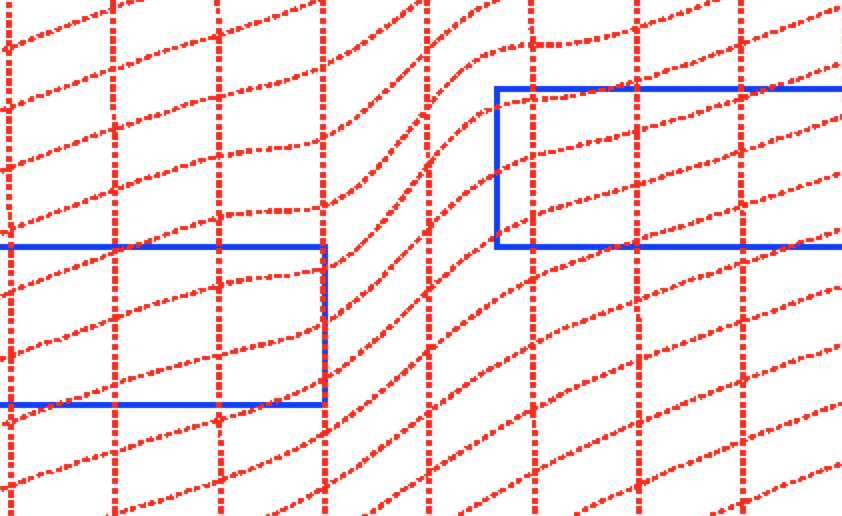
\includegraphics[width=6cm, height=3cm]{TPS_withnormals}
\caption{}
\end{subfigure}
\caption{The demonstration scene (top image) has two suturing pads aligned in the same horizontal plane. In the test scene (bottom two images) the right pad is shifted upwards. (a) Warp found by TPS using six pairs of correspondence points between the scenes, indicatd by the magenta points. (b) Warp found by TPS after adding in correspondence points along the relevant normals, indicated by the green points. The second warp is more likely to effectively generalize trajectories as it better captures the structure of scene.}
\label{fig:normals}
\end{figure}
When using thin plate splines to generalize manipulation trajectories fails, it is often because the warping function that is found does not preserve important geometric properties of the scene. A common failure mode arises because the warping function fails to preserve surface normals. For example, consider the manipulation task of suturing two pads of tissue. One important aspect of this task is the suturing needle's angle of entry into the pads. However, in situations where the pads are offset vertically relative to the demonstration, the warping function that minimizes error on the correspondence points rarely captures this. Figure~\ref{fig:normals} shows a two dimensional illustration of this problem. One approach for making this trajectory transfer more robust is to include correspondences on surface normals. As an initial investigation, we model this type of constraint by introducing new point correspondences to model the surface normals, shown in Figure~\ref{fig:normals}. We found through experimenting with this approach that it leads to interpolating splines that generalize demonstrations more effectively. 

However, we would like to find a more principled way to incorporate these surface normal correspondences into the thin plate spline optimization. Formally, we want to find a mapping between $m$ normals \ns{l}, $l=1,...,m$, at respective positions \xes{l} in the source scene, and the respective normals \nt{l} in the target scene. A natural way to map a surface normal (or any vector) through a function like this is to make use of the tangent space. In differential geometry, this is the idea of a pushforward operator~\cite{ralph1978foundations}. In our setting, mapping a normal $\ns{l}$ through a thin plate spline function $f$ at a point $\xes{l}$ corresponds to multiplying by $J_f(\xes{l})$, the Jacobian of $f$ at $\xes{l}$: $$J_f(\xes{l}) \cdot \ns{l}.$$  

Thus, correspondences between normals in two scenes result in constraints on the Jacobian of $f$, while correspondences between points result in constraints on the value of $f$. Incorporating this into the thin plate spline objective, we get the following problem:
\begin{equation}
\begin{align}
 &\underset{f}{\text{minimize\ \ \ }} & ||f||_{tps}^2 \\
 &\text{subject to\ \ \ }
 & \xt{i} = f(\xs{i}) \\
 && \nt{l}= J_f(\xes{l}) \cdot \ns{l}\\
\end{align}
.
\label{eq:tps_normals}
\end{equation}

Alternatively, we can trade off between the error on the correspondences and the smoothness of our curve with the following objective
\begin{equation}
f = \underset{f}{\text{argmin}} \sum_{i=1}^k ||\xt{i} - f(\xs{i})||_2^2 + \sum_{l=1}^m ||\nt{l} - J_f(\xes{l}) \cdot \ns{l}||_2^2 + \lambda ||f||_{tps}^2.
\label{eq:tps_normals_reg}
\end{equation}

Bookstein and Green show an approximation method to solve Equation~\ref{eq:tps_normals}, in which $f$ can be expressed as a weighted sum of slope functions and the landmark-only TPS basis functions $\mathbf{b}$~\cite{BooksteinGreen}. The slope functions $U_{\mathbf{t}$ are the derivative of $U$ in the direction $\mathbf{t}$. In 2D, we have
\begin{equation}
\begin{align*}
U_{\mathbf{t_i}}(\mathbf{x}) &= \mathbf{t_i} \cdot \nabla U(\mathbf{x}) \\
&= (2 \ln ||\mathbf{x}|| + 1)(\mathbf{x} \cdot \mathbf{t_i}) .
\end{align*}
\end{equation}

Then $f$ can be written as
\begin{equation}
f(\mathbf{x}) =
E^\top
\begin{bmatrix} 
  \mathbf{b}^\top &
  -U_{\ns{1}}(\mathbf{x}-\xes{1}) &
  -U_{\ns{2}}(\mathbf{x}-\xes{2}) &
  \cdots &
  -U_{\ns{m}}(\mathbf{x}-\xes{m})
\end{bmatrix}^\top
\end{equation}
where $E$ is the weight matrix that minimizes the objective in Equation~\ref{eq:tps_normals}. Recall that $\mathbf{b}$ has the landmark-only TPS basis fuctions
\begin{equation}
\mathbf{b} =
\begin{bmatrix} 
  U(\mathbf{x} - \xs{1}) & U(\mathbf{x} - \xs{2}) & \cdots & U(\mathbf{x} - \xs{k}) & \mathbf{x}^\top & 1
\end{bmatrix}^\top .
\end{equation}



\section{Clustering \& Lookahead}

\begin{figure}
\centering
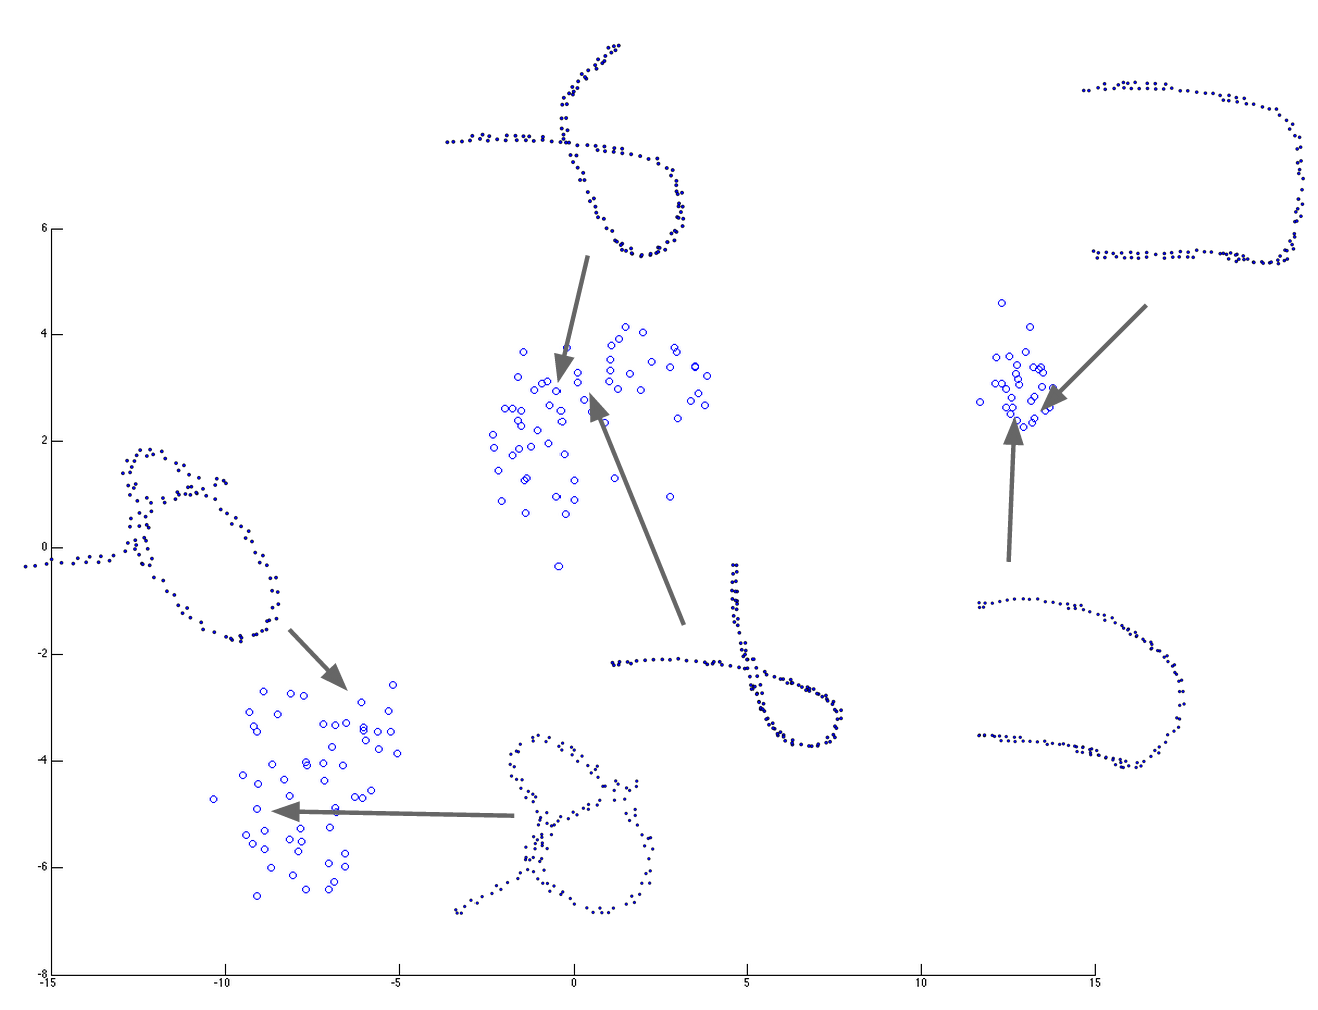
\includegraphics[width=0.5\textwidth]{tsne_clusters}
\caption{Two-dimensional t-SNE of rope configurations.}
\label{fig:tsne_clusters}
\end{figure}

The TPS registration error provides a distance metric with which we can evaluate the similarity of scene configurations. This means that by using any kernel such as a Gaussian RBF, we can run a kernelized $k$-means clustering algorithm~\cite{Dhillon2004} to separate the start configurations of demonstrations into distinct clusters. Thus, by setting only a few parameters (the number of clusters and the parameters of the kernel function), we can derive structure from known scene configurations and demonstrations. In effect, we are grouping specific scene configurations into $k$ well-known, commonly encountered abstract states, and the provided demonstrations then constitute transitions between these states.

For the knot-tying scenario, visualizing these clusters using a low-dimensional embedding such as t-SNE~\cite{tSNE2008} demonstrates that this method of clustering is able to effectively separate the scene configurations into three clusters, as shown in Figure~\ref{fig:tsne_clusters}. Additionally, examining the rope configurations present within each cluster indicates that each cluster represents a distinct step along this particular rope-tying method.

These clusters also provide us an effective means of quantifying how effectively we can proceed from a given state. For a new scene configuration, we can find its $k$ nearest neighbors out of the provided demonstration start configurations. We then create a histogram of the clusters of these $k$ demonstrations, and take the maximum count as a score. We call this score the \emph{consensus score} and use it as a measure of how likely we are to succeed from a given scene configuration. Intuitively, a higher consensus score is better because it is easier to generalize to scene configurations that lie in the interior of clusters. For configurations that satisfy this property, there exist many demonstrations that operate on similar configurations, which indicates that this configuration is not extraordinary or unexpected and provides many valid demonstrations to choose from. On the other hand, points that are far away from these clusters are troublesome, since none of the existing demonstrations operate on similar configurations.

If we allow ourselves to assume domain-specific knowledge, we can leverage this clustering to steer ourselves towards rope configurations that are well covered by demonstrations. In particular, if we have access to a rudimentary simulation of the test environment, then we can perform lookahead to avoid states that are poorly understood. Given a set of demonstrations to generalize, we can compute nearest-neighbors using registration cost as a similarity measure. If a state's highest ranked nearest neighbors all belong to the same cluster, we say there is a high consensus score for that state. If the consensus score is below some threshold, we can simulate candidates and take the demonstration which, after simulation, has the highest consensus score. In applying this heuristic, we bias our search to stay on the interior of our learned clusters. In practice, we found that there were many scenarios where this heuristic was able to avoid dead ends that blocked nearest-neighbor. Figure~\ref{fig:lookahead_results} illustrates one such scenario. Note that simply using minimum or mean registration cost as a search heuristic will likely lead to failure: there are many cases where executing the best demonstration (the demonstration that leads to tying a knot in the fewest steps) yields a higher registration cost than an alternative. 

\begin{figure}
\centering
\begin{subfigure}[b]{.24\textwidth}
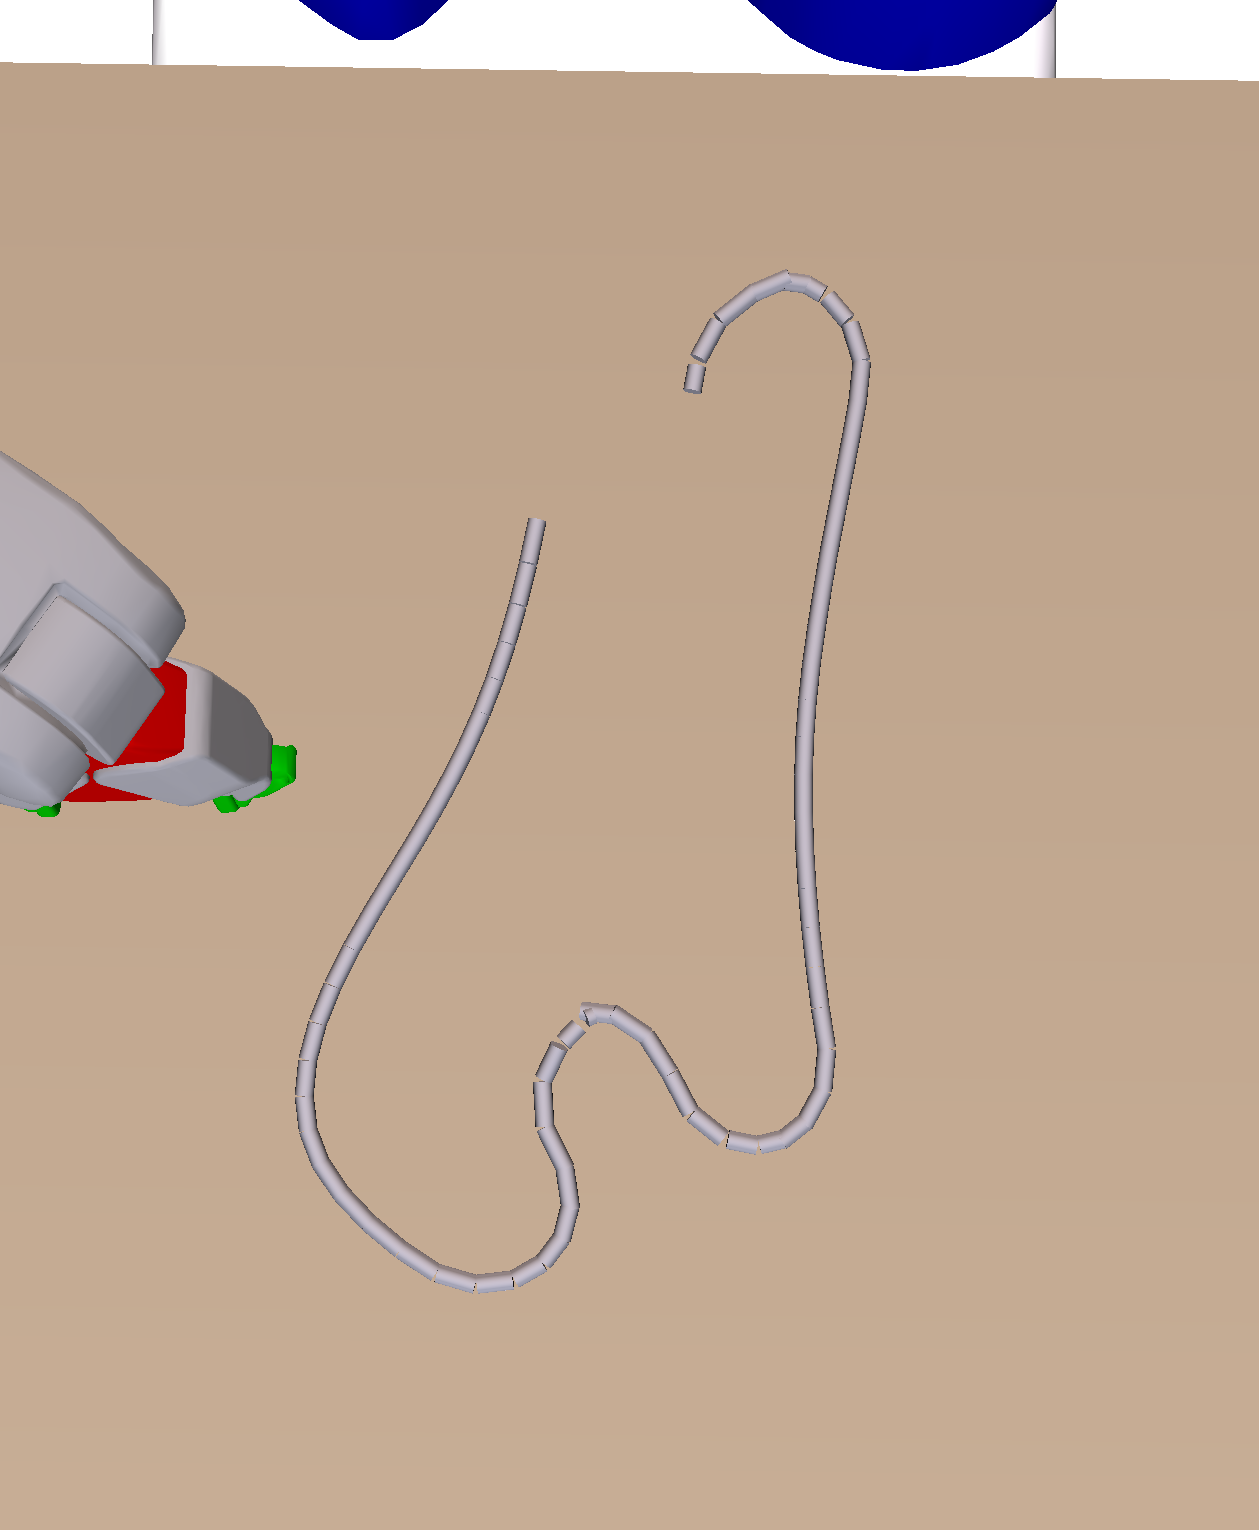
\includegraphics[width=\textwidth]{no_lookahead_fail_start.png}
\caption{}
\end{subfigure}
\begin{subfigure}[b]{.24\textwidth}
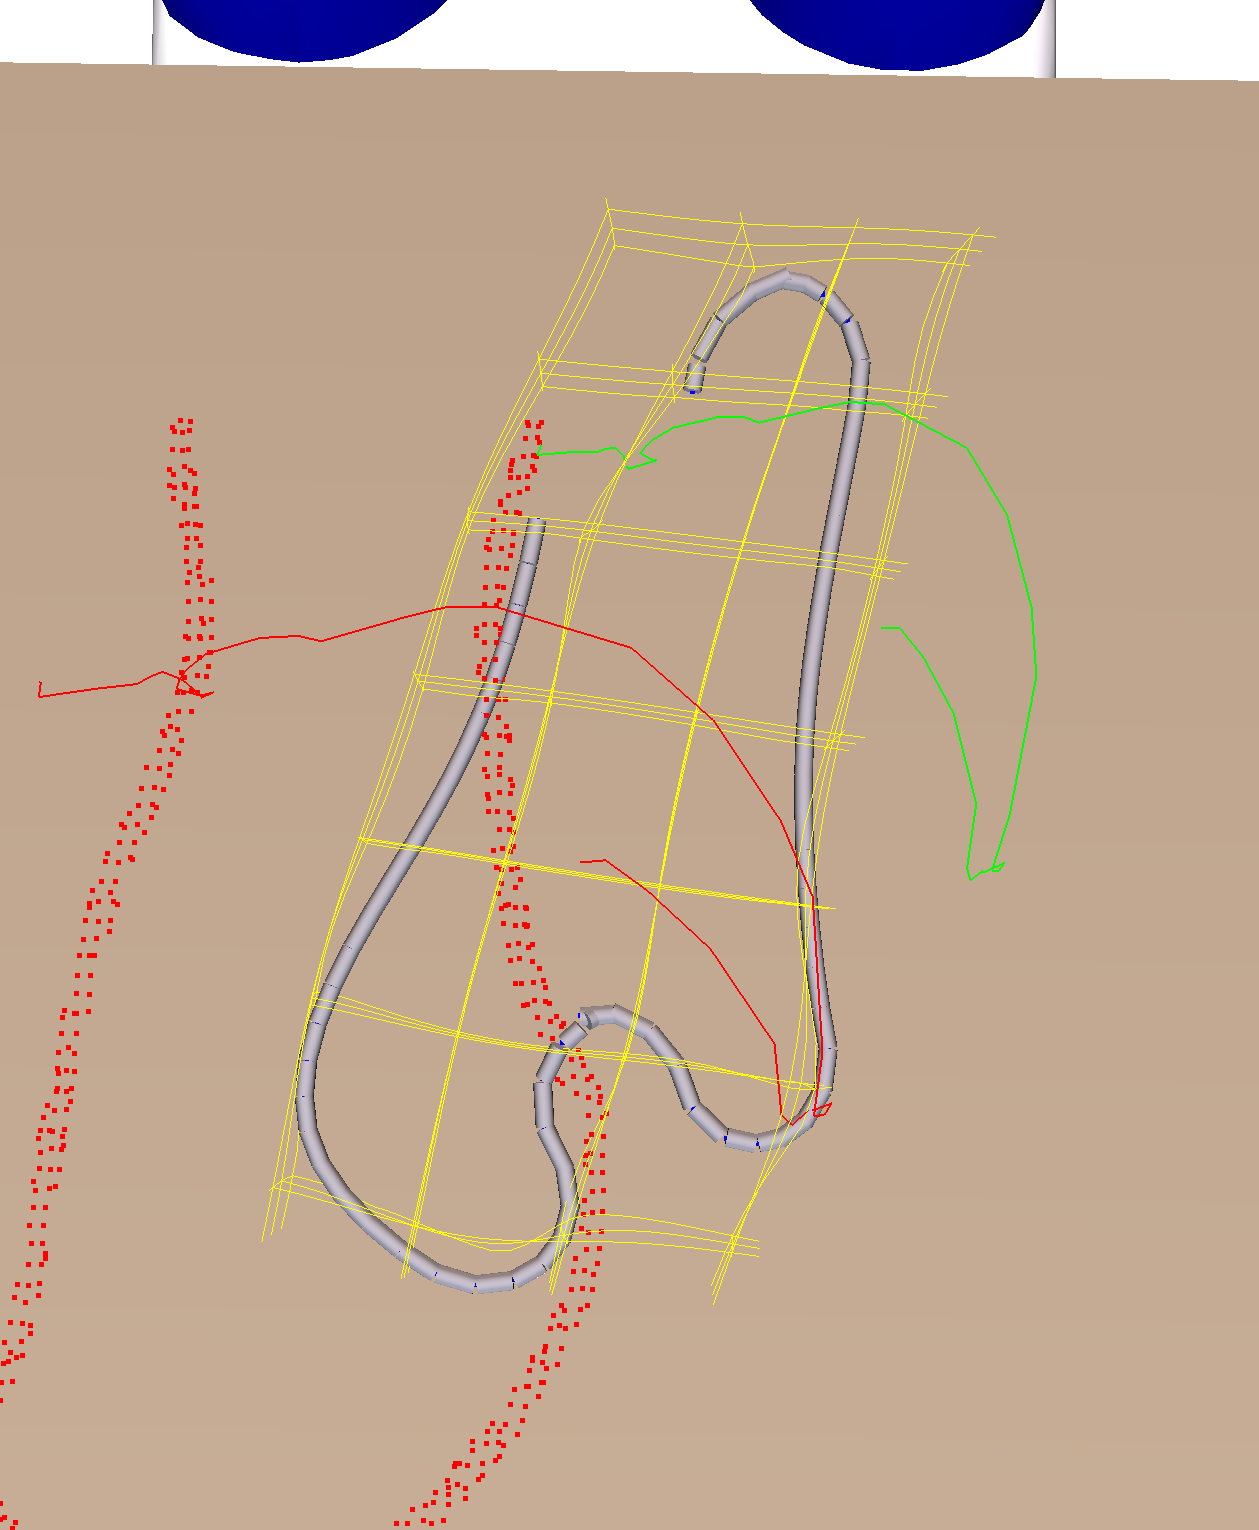
\includegraphics[width=\textwidth]{sim_res1.png}
\caption{}
\end{subfigure}
\begin{subfigure}[b]{.24\textwidth}
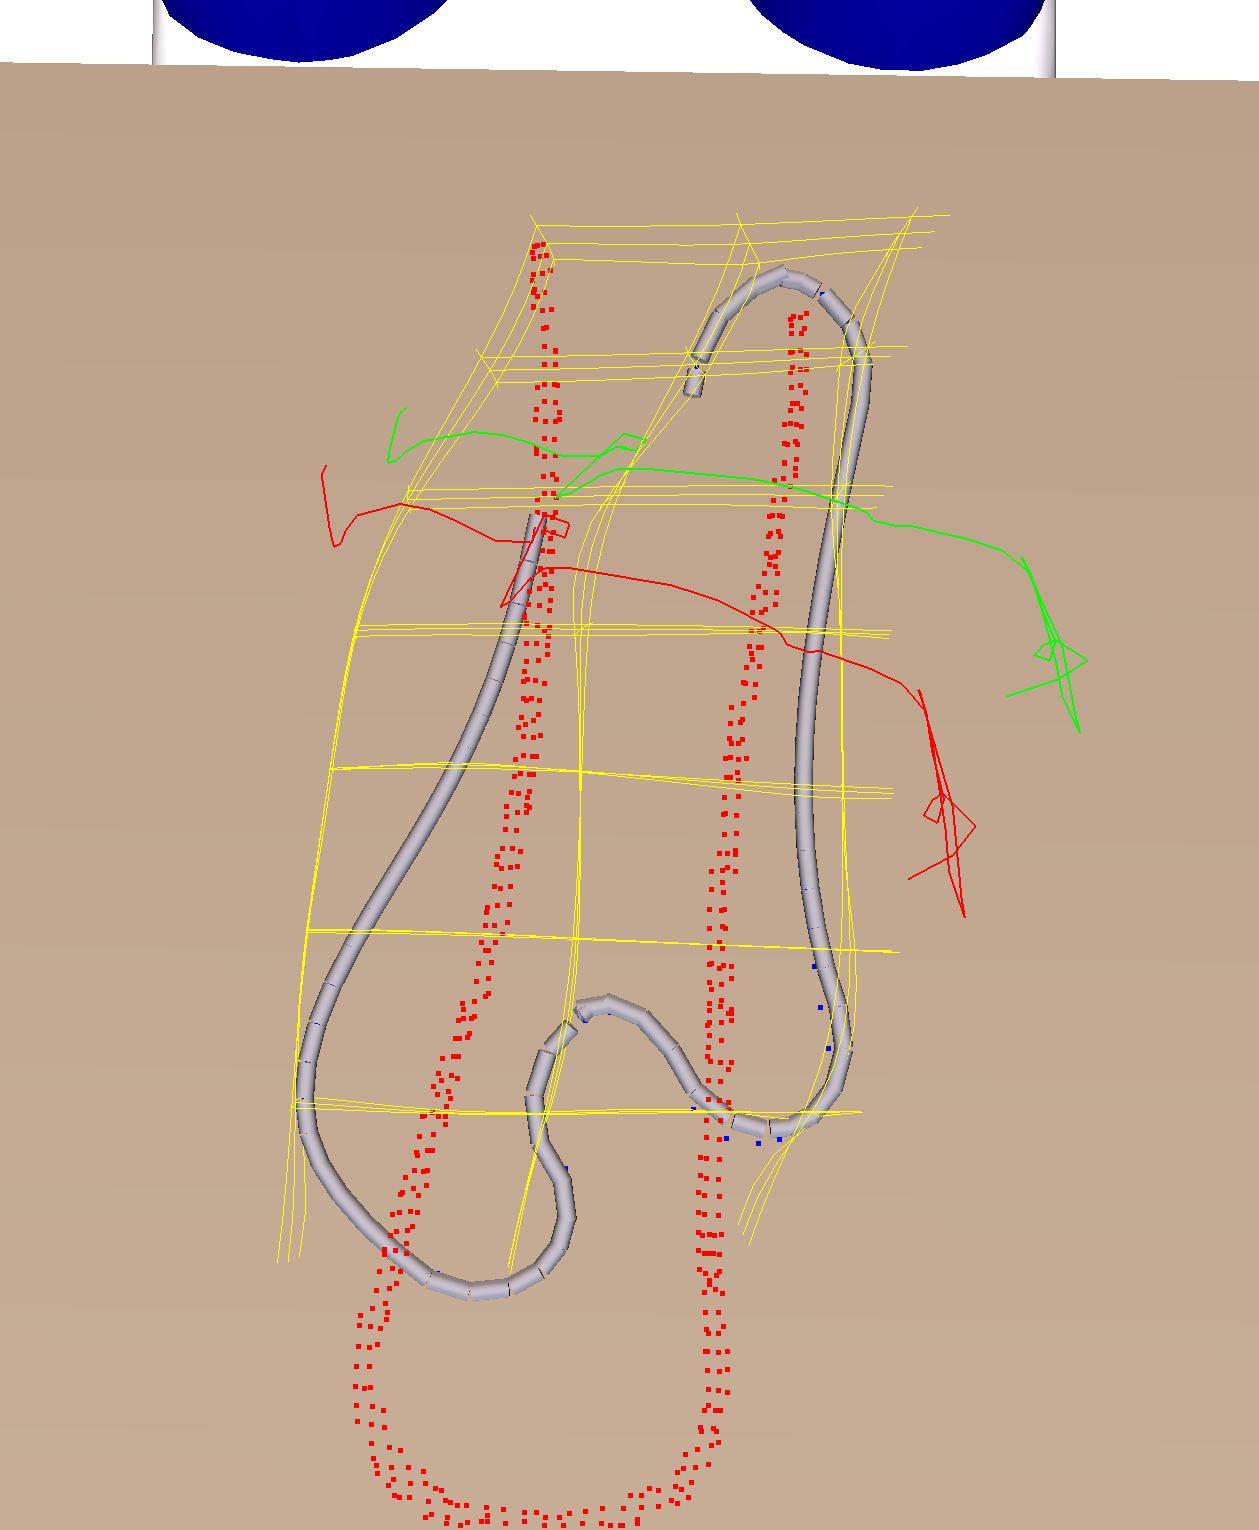
\includegraphics[width=\textwidth]{sim_res2.png}
\caption{}
\end{subfigure}
\begin{subfigure}[b]{.24\textwidth}
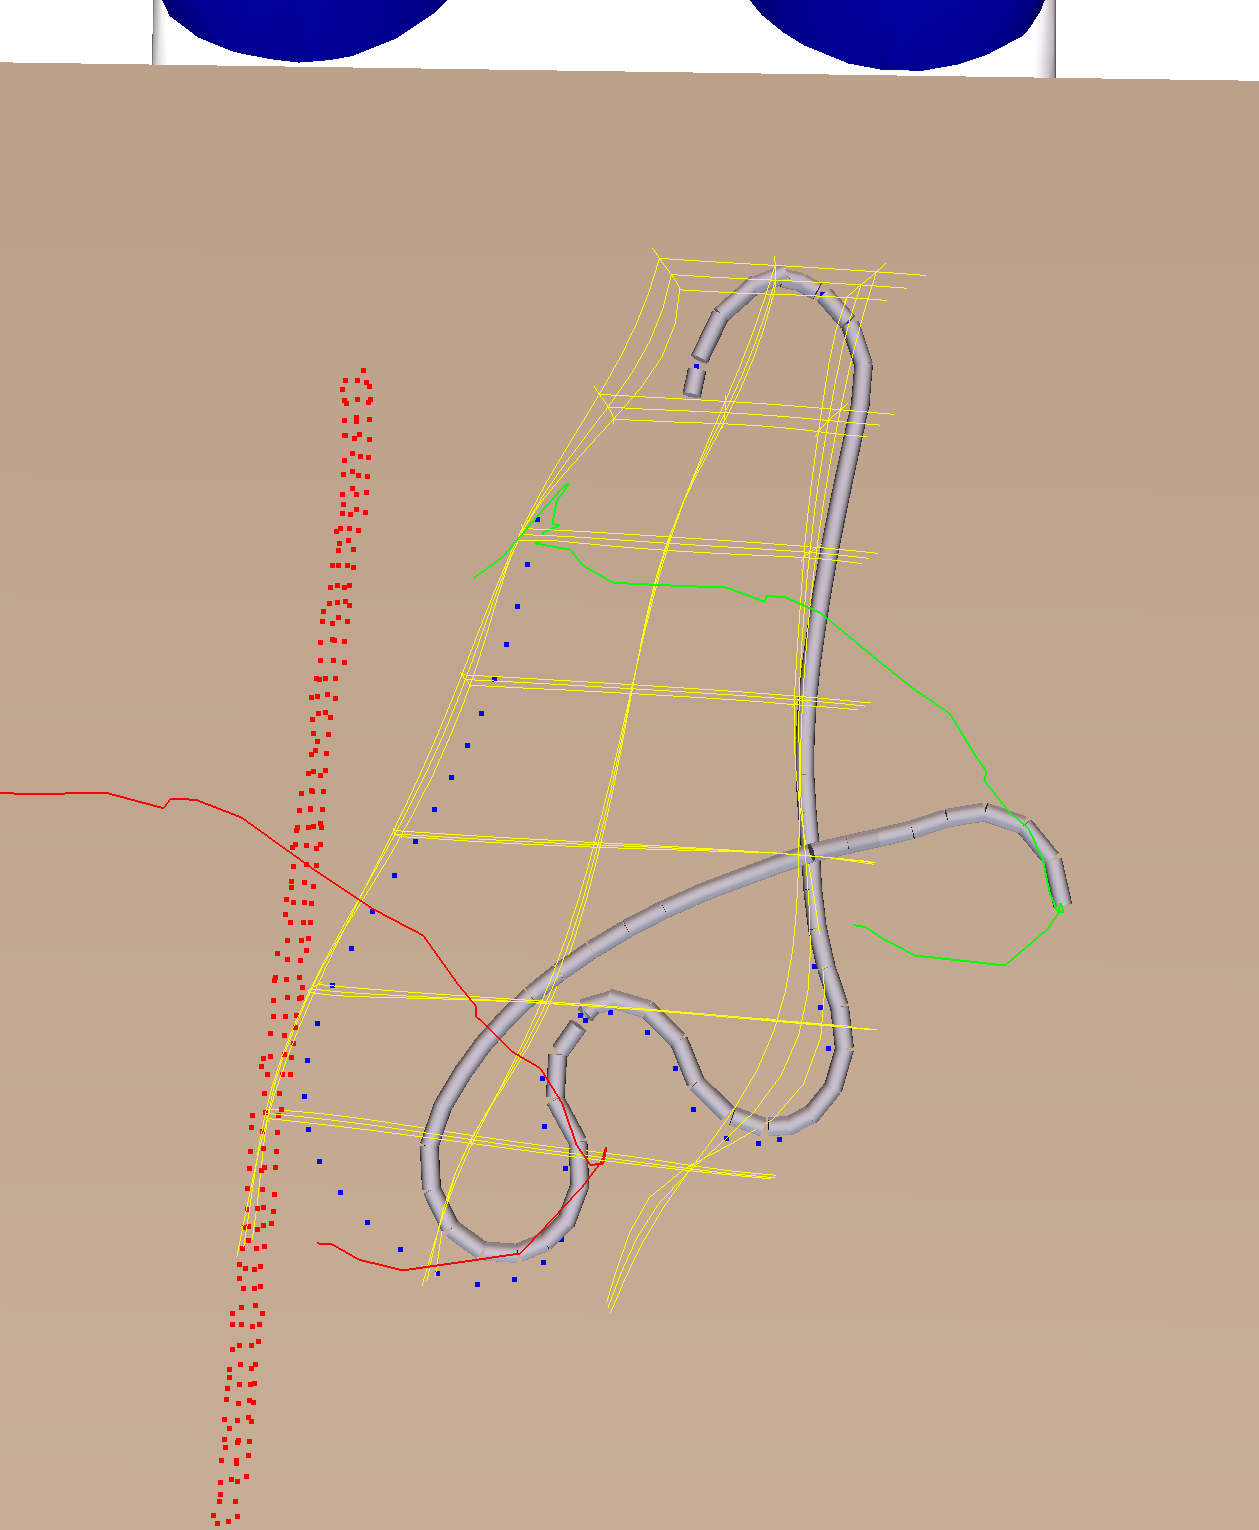
\includegraphics[width=\textwidth]{sim_res3.png}
\caption{}
\end{subfigure}\\
\caption{(a): Initial state for a simulation run where lookahead succeeds, but nearest-neighbor does not. (b)-(c): States that result from simulating the two best nearest neighbors according to registration cost. The green path illustrates the path the gripper took. It misses the rope entirely, so the next state is the same as the initial state. (d): Simulation result from using the 3rd best demonstration according to registration cost. This demonstration is the one chosen by our heuristic and results in a successful knot-tie.}
\label{fig:lookahead_results}
\end{figure}

\section{Limitations and Future Work}

We are currently implementing our unified objective for simulations of three-dimensional tasks, in particular rope-tying and suturing. Our hope is that this will either provide convincing evidence that the unified formulation produces and selects better trajectories, or it will provide new insight with which we can revise our approach. In addition, our current approach for incorporating surface normals is approximate. To formally incorporate normals into the optimization, we are implementing a reformulation of the TPS objective that incorporates first-order constraints~\cite{BooksteinGreen}.

There is also an interesting avenue of research based on a more explicit modelling of the underlying MDP that our robot is acting in. In this setting, the state space is the set of paired configurations of the robot and rope. The space of actions is a discrete set, with one action corresponding to each demonstration. This formalism lets us apply techniques such as reinforcement learning or inverse reinforcement learning to learn a Q-function for each action. Such approaches would enable us to learn which demonstrations generalize well and discover, on a per demonstration basis, which rope states each demonstration is most applicable to.

Estimating scene correspondences more accurately is also crucial for improving demonstration selection. Schulman et al. use the TPS-RPM approach to estimate correspondences between point clouds of the demonstration scene and the new scene. TPS-RPM only takes into account the positions of the points, and requires a one-to-one correspondance between the points in the two point clouds. However, there may be outliers, points in the demonstration scene that do not correspond to any in the new scene or vice versa. Using computer-vision based features, such as SIFT and shape contexts, has the potential to detect these outliers and improve estimation of point correspondences.

\section{Conclusion}

We have presented several approaches for improving the transfer of trajectories to new scenarios when multiple demonstrations are available. We improve the robustness of trajectory transfer by jointly optimizing for both a smooth warping function and a feasible trajectory, as well as incorporating surface normal correspondences. Leveraging clustering allows us to use lookahead to predict how likely applying a certain transferred trajectory will result in success, which improves demonstration selection. Finally, we have provided examples which convincingly demonstrate that our proposed extensions improve robustness of the trajectory transfer method.

\bibliographystyle{unsrt}
\bibliography{references}

\end{document}

